% Chapter 5

\chapter{The pairing and chemical potentials} % Main chapter title

\label{Chapter5} % For referencing the chapter elsewhere, use \ref{Chapter5} 

\lhead{Chapter 5. \emph{Pairing and chemical potentials}} % This is for the header on each page - perhaps a shortened title

%----------------------------------------------------------------------------------------
In this chapter we will first derive an integral equation for the pairing potentials, the socalled gap equation. This is done in section \ref{sec.pairingpotential.integralequation}. Next we consider the chemical potential. Fundamentally the interaction of the fermions will alter the chemical potential from the one for the free gas. This is taken into acount by virtue of the number equation. See section \ref{sec.chemicalpotential.numberequation}. As a result, we will have \textit{two} integral equations for the \textit{two} potentials, and we can solve for both simultaneously. The numerical calculations are then done in section \ref{sec.pairingandchemicalpotential.numericalcalculation}. 

\section{The gap equation} \label{sec.pairingpotential.integralequation}
In this section we find an integral equation for the pairing potential $\Delta_k$, known as the gap equation. Inspecting the definition in equation \eqref{eq.pairingpotentialdef} we see, that we need to calculate $\langle f_k f_{-k} \rangle$, which in turn specifies another term in the Hamiltonian: $\langle f^\dagger_k f^\dagger_{-k} \rangle$. From the transformation defined in equation \eqref{eq.fermionquasiparticledef}, we get that $f_k = u^*_{F,k}\zeta_k - v_{F,k}\zeta^\dagger_{-k}$ and $f_{-k} = v_{F,k}\zeta^\dagger_k + u^*_{F,k}\zeta_{-k}$. Hereby:
\begin{align}
\langle f_k f_{-k} \rangle &= \left \langle (u^*_{F,k}\zeta_k - v_{F,k}\zeta^\dagger_{-k}) (v_{F,k}\zeta^\dagger_k + u^*_{F,k}\zeta_{-k}) \right \rangle = u^*_{F,k}v_{F,k}\left[ \left \langle \zeta_k \zeta^\dagger_{k} \right \rangle - \left \langle \zeta^\dagger_{-k} \zeta_{-k} \right \rangle \right]  \nonumber \\
& =  u^*_{F,k}v_{F,k}\left[ 1 - \left \langle \zeta^\dagger_{k} \zeta_k \right \rangle - \left \langle \zeta^\dagger_{-k} \zeta_{-k} \right \rangle \right] = u^*_{F,k}v_{F,k}\left[1 - 2f(E_{F,k})\right], \nonumber
\end{align}
where we in the last equality use, that $\left \langle \zeta^\dagger_{k} \zeta_{k} \right \rangle = f(E_{F,k})=(\exp(\beta E_{F,k})+1)^{-1} $. Inserting this into the expression for $\Delta_k$ and using the relation $\frac{v_{F,k}\Delta^*_k}{u_{F,k}}=E_{F,k}-\varepsilon_k$ from equation \eqref{eq.Kitaev.uk_vk} we get the gap equation as a sum:
\begin{equation}
\Delta_k = - \frac{1}{\mathcal{L}}\sum_{k'} W^\text{ind}_{FF}(k,k')\frac{\Delta_{k'}}{2E_{F,k'}}\tanh\left(\frac{\beta E_{F,k'}}{2}\right).
\label{eq.GapequationSum}
\end{equation} 
As mentioned in the start of chapter \ref{Chapter2}, we use periodic boundary conditions of the string to investigate the bulk properties. This means, that the spacing of the $k$-points are $dk = \frac{2\pi}{\mathcal{L}}$, and so we can transform the above into the following integral:
\begin{equation}
\Delta_k = - \int \frac{dk'}{2\pi} W^\text{ind}_{FF}(k,k')\frac{\Delta_{k'}}{2E_{F,k'}}\tanh\left(\frac{\beta E_{F,k'}}{2}\right), 
\label{eq.GapequationIntegral}
\end{equation} 
and hereby canceling the length $\mathcal{L}$. Because of the symmetries of the coupling potential summarized in equation \eqref{eq.CouplingPotentialSymmetries}, we see, that $W^\text{ind}_{FF}(0,k') = 0$. Hence, it is immediately clear from both equation \eqref{eq.GapequationSum} and \eqref{eq.GapequationIntegral}, that $\Delta_{k=0} = 0$ for any temperature. This means, that $E_{F,k=0} = |\mu| > 0$. This means, that $\frac{E_{F,k}}{|k|}$ blows up for $k\to 0$. Hence, it must further be the case, that $v_c = \min_k \frac{E_{F,k}}{|k|} > 0$. The Landau criterion for superfluidity, as discussed in section \ref{sec.Superfluidity}, is therefore fulfilled. The exact value of $v_c$ requires a further analysis. 

Written out in the $l_t \to 0$ limit and with unitless quantities denoted by tildes, the gap integral is:
\begin{equation}
\tilde{\Delta}_{\tilde{k}} = \frac{2}{\pi^3}\frac{n_B}{n_F^3}(k_Fa_{BF})^2\left(\frac{m_F}{m_B} + \frac{m_B}{m_F}+ 2\right) \int_0^\infty d\tilde{k}' \; \ln\left[\frac{(\tilde{k}+\tilde{k}')^2+2/\tilde{\xi}^2}{(\tilde{k}-\tilde{k}')^2+2/\tilde{\xi}^2}\right] \frac{\tilde{\Delta}_{\tilde{k}'}}{\tilde{E}_{F,\tilde{k}'}}\tanh\left[\frac{\tilde{E}_{F,\tilde{k}'}}{2\tilde{T}}\right],
\label{eq.GapequationIntegralUnitless}
\end{equation} 
where $\tilde{\xi} = k_F\xi = \frac{\pi}{\sqrt{8 n_B/n_F^3 k_Fa_B}}$, and $\tilde{E}_{F,\tilde{k}} = \sqrt{(\tilde{k}^2-\tilde{\mu})^2 + |\tilde{\Delta}_{\tilde{k}}|^2}$. We have also made use of the fact, that the integrand is even i $\tilde{k}'$. Notice, that since we are neglecting retardation effects, we assume $\left(\frac{m_F}{m_B}\right)^2\frac{4}{\pi^2}\frac{n_B}{n_F^3}k_Fa_B \gg 1$ as discussed in section \ref{sec.RetardationEffects}. If the stronger condition, that $\frac{n_B}{n_F^3}k_Fa_B \gg 1$ is fullfilled, we see that we are only investigating short ranged interactions between the fermions, since $k_F\xi \ll 1$ in this limit. 

\section{The number equation} \label{sec.chemicalpotential.numberequation}
In this section we use the number equation to derive a second integral equation for the chemical and pairing potentials. The number equation is: $N_F = \sum_k \left \langle f_k^\dagger f_k \right \rangle$, where we average with respect to the thermalized state of the system. From earlier we know, that $f_k = u_{F,k}^* \zeta_k -v_{F,k} \zeta_{-k}^\dagger$. This leads to the sum formula:
\begin{equation}
N_F = \sum_k \left(|u_{F,k}|^2-|v_{F,k}|^2\right) f(E_{F,k}) + |v_{F,k}|^2,\nonumber
\end{equation}
where $f(E_{F,k}) = (\exp(\beta E_{F,k}) + 1)^{-1}$ is the distribution of the fermion quasiparticles. Using the expression for the $u$ and $v$ coefficients, we get:
\begin{equation}
n_F = \int \frac{dk}{2\pi} \frac{\varepsilon_k}{E_{F,k}}f(E_{F,k}) + \frac{1}{2}\left(1 - \frac{\varepsilon_k}{E_{F,k}}\right), \nonumber
\end{equation}
where $n_F = N_F/\mathcal{L}$. For the free fermion gas $k_F = n_{F,0}\pi$. Since we consider $N_F$ and $\mathcal{L}$ as constant $n_F = n_{F,0}$. By going to unitless quantities, we hereby obtain:
\begin{equation}
1 = \int_0^\infty d\tilde{k} \; \frac{\tilde{\varepsilon}_{\tilde{k}}}{\tilde{E}_{F,k}}\frac{1}{\text{e}^{ \tilde{E}_{F,\tilde{k}}/\tilde{T} } + 1 } + \frac{1}{2}\left(1 - \frac{\tilde{\varepsilon}_{\tilde{k}}}{\tilde{E}_{F,\tilde{k}}}\right). 
\label{eq.NumberEquationUnitless}
\end{equation}
This gives us the required second equation.


\section{Calculating the pairing potential} \label{sec.pairingandchemicalpotential.numericalcalculation}
\subsection{Assumptions}
Before performing the numerical calculation, it is worthwhile to summarize what assumptions, we have made so far. To trap the fermions in one dimension we assumed, that the transverse energy, $\omega_t$, is much larger than the typical energy of the fermions, $\epsilon_{F,0}$. This lead to requirement in the first line of table \ref{tab.assumptions}. To have neglible ground state depletion of the condensate, we saw in equation \eqref{eq.excitedbosonsBEC}, that we needed to assume $(n_Ba_B^3)^{1/3}\ll 1$. This is line two of the table. Further, to be able to neglect retardation effects, we needed to assume, that the fermions moves slowly relative to the quasiparticles in the BEC. This is line 3 in the table. Finally, to ensure that we only need to work to first order in the Bose-Fermi interaction strength $g_{BF}$, we need $(n_Ba_{BF}^3)^{1/3} \ll 1$. This is line 4 of the table. 

\begin{table}[htb]
\centering
\caption{\textit{Summary of the assumptions made so far. $m_r = \frac{m_Fm_B}{m_F+m_B}$ is the reduced mass. B and F refer to Bosons and Fermions respectively. $\omega_n$ is the bosonic Matsubara frequencies associated with the induced interaction.}}
\begin{tabular}{|l|l|r|l|}
\hline \textbf{Quantity} & \textbf{Parameters} 						& \textbf{Assumption}						& \textbf{Reason}	\\
\hline Transverse energy gap & $\omega_t = \frac{1}{\sqrt{m_Fl_t}}$ & $(k_Fl_t)^2/2 	\ll 1$ 					& Trap in transverse ground state \\
\hline B-B scattering length & $g_B = \frac{4\pi a_B}{m_B}$			& $(n_Ba_B^3)^{1/3}	\ll 1$					& Negligible BEC depletion  \\
\hline $\omega_n = 0$ limit  & $v_F,c_0$							& $v_F/c_0 \ll 1$ & Negligible retardation effects  \\
\hline B-F scattering length & $g_{BF} = \frac{2\pi a_{BF}}{m_r}$ 	& $(n_Ba_{BF}^3)^{1/3}	\ll 1$				& Simple diagrammatics\\
\hline 
\end{tabular}
\label{tab.assumptions}
\end{table}

\subsection{Momentum and temperature dependency of the pairing}
In this subsection we will describe and perform a numerical calculation of the momentum and temperature dependency of the pairing. The chemical potential is used to enhance the accuracy of the solution for the pairing, but is else not our focus. 

The numerical calculation is based on the following idea. We start at $T = 0$ and make an initial guess for $\Delta_k$ and $\mu(T=0)$. Then we plug this into the gap equation \eqref{eq.GapequationIntegralUnitless} for $\beta = 1/k_BT = \infty$ and hereby obtain a better result for $\Delta_k(T=0)$. This is then inserted into the number equation \eqref{eq.NumberEquationUnitless}, whereby we get an updated guess for the chemical potential. The process is repeated until the maximum of $\Delta_k(T=0)$ \textit{and} the Fermi energy $\mu( T=0 )$ does not change by more than $1$\textperthousand. Afterwards we increase the temperature with a small increment $dT$ and use $\Delta_k(T=0)$ and $\mu( T=0 )$ as an initial guesses repeating the process for $T=0$. This is done for rising temperatures until we reach some critial temperature, where $\Delta_k(T_c)\approx 0$ for all $k$, somewhat equivalent to the original BCS-theory\cite{Tinkham,LandauStatPhys2,PlischkeStatPhys}. The procedure is quite slow, because we need the entire function $\Delta_k$ for each $k$-value in the iteration. Finally, we will use the $l_t \to 0$ limit for the coupling potential from equation \eqref{eq.CouplingPotentiallt=0} and so the gap equation of interest is equation \eqref{eq.GapequationIntegralUnitless}. It is possible to come with some rather well educated initial guesses for the pairing and the chemical potentials. We expect, that the chemical potential is not altered significantly from the one for the free gas, and so $\tilde{\mu}(T = 0) = 1$ is a good initial guess. The pairing needs to be odd in $k$ and by inspecting the integral equation, we see that we only get significant contributions around $\tilde{k}' = \tilde{k}$. Hence, we expect that the pairing goes to 0 for large values of $\tilde{k}$.  

An increasing number of iterations are needed near the transition from the superfluid to normal phase. Near the transition temperature $T_c$ the maximal pairing has the asymptotic form:
\begin{equation}
\frac{\max_{k}[\Delta_k(T)]}{\epsilon_{F,0}} \approx \max_k[\Delta_{k}(T=0)]\frac{T}{T_F}\left[1 - \left(\frac{T}{T_c}\right)^3\right]^{1/2}. 
\label{eq.maxpairingasymp}
\end{equation}
This resembles the original BCS-theory apart from the power of 3 of $\frac{T}{T_c}$. Near $T_c = 0.129 T_F$ the numerical calculation needs an increasing number of iterations. We therefore halt the calculation above $T_c$ and set $\Delta_k = 0$ for all $k$. This leads to the figures \ref{fig.Deltakkdepend} and \ref{fig.maxkDeltakTdepend}. From here we get, that $\max_{k,T}[\Delta_k(T)]/\epsilon_F \approx 0.280$. It follows, that the maximal gap to critical temperature ratio is for the present calculation is: $\max_{k,T}[\Delta_k(T)]/(k_B T_c) \approx 2.16$. This is similar to the BCS-value of $1.77$ \cite{BruusFlensberg}.  

\begin{figure} 
\begin{center}  
% GNUPLOT: LaTeX picture with Postscript
\begingroup
  \makeatletter
  \providecommand\color[2][]{%
    \GenericError{(gnuplot) \space\space\space\@spaces}{%
      Package color not loaded in conjunction with
      terminal option `colourtext'%
    }{See the gnuplot documentation for explanation.%
    }{Either use 'blacktext' in gnuplot or load the package
      color.sty in LaTeX.}%
    \renewcommand\color[2][]{}%
  }%
  \providecommand\includegraphics[2][]{%
    \GenericError{(gnuplot) \space\space\space\@spaces}{%
      Package graphicx or graphics not loaded%
    }{See the gnuplot documentation for explanation.%
    }{The gnuplot epslatex terminal needs graphicx.sty or graphics.sty.}%
    \renewcommand\includegraphics[2][]{}%
  }%
  \providecommand\rotatebox[2]{#2}%
  \@ifundefined{ifGPcolor}{%
    \newif\ifGPcolor
    \GPcolorfalse
  }{}%
  \@ifundefined{ifGPblacktext}{%
    \newif\ifGPblacktext
    \GPblacktexttrue
  }{}%
  % define a \g@addto@macro without @ in the name:
  \let\gplgaddtomacro\g@addto@macro
  % define empty templates for all commands taking text:
  \gdef\gplbacktext{}%
  \gdef\gplfronttext{}%
  \makeatother
  \ifGPblacktext
    % no textcolor at all
    \def\colorrgb#1{}%
    \def\colorgray#1{}%
  \else
    % gray or color?
    \ifGPcolor
      \def\colorrgb#1{\color[rgb]{#1}}%
      \def\colorgray#1{\color[gray]{#1}}%
      \expandafter\def\csname LTw\endcsname{\color{white}}%
      \expandafter\def\csname LTb\endcsname{\color{black}}%
      \expandafter\def\csname LTa\endcsname{\color{black}}%
      \expandafter\def\csname LT0\endcsname{\color[rgb]{1,0,0}}%
      \expandafter\def\csname LT1\endcsname{\color[rgb]{0,1,0}}%
      \expandafter\def\csname LT2\endcsname{\color[rgb]{0,0,1}}%
      \expandafter\def\csname LT3\endcsname{\color[rgb]{1,0,1}}%
      \expandafter\def\csname LT4\endcsname{\color[rgb]{0,1,1}}%
      \expandafter\def\csname LT5\endcsname{\color[rgb]{1,1,0}}%
      \expandafter\def\csname LT6\endcsname{\color[rgb]{0,0,0}}%
      \expandafter\def\csname LT7\endcsname{\color[rgb]{1,0.3,0}}%
      \expandafter\def\csname LT8\endcsname{\color[rgb]{0.5,0.5,0.5}}%
    \else
      % gray
      \def\colorrgb#1{\color{black}}%
      \def\colorgray#1{\color[gray]{#1}}%
      \expandafter\def\csname LTw\endcsname{\color{white}}%
      \expandafter\def\csname LTb\endcsname{\color{black}}%
      \expandafter\def\csname LTa\endcsname{\color{black}}%
      \expandafter\def\csname LT0\endcsname{\color{black}}%
      \expandafter\def\csname LT1\endcsname{\color{black}}%
      \expandafter\def\csname LT2\endcsname{\color{black}}%
      \expandafter\def\csname LT3\endcsname{\color{black}}%
      \expandafter\def\csname LT4\endcsname{\color{black}}%
      \expandafter\def\csname LT5\endcsname{\color{black}}%
      \expandafter\def\csname LT6\endcsname{\color{black}}%
      \expandafter\def\csname LT7\endcsname{\color{black}}%
      \expandafter\def\csname LT8\endcsname{\color{black}}%
    \fi
  \fi
    \setlength{\unitlength}{0.0500bp}%
    \ifx\gptboxheight\undefined%
      \newlength{\gptboxheight}%
      \newlength{\gptboxwidth}%
      \newsavebox{\gptboxtext}%
    \fi%
    \setlength{\fboxrule}{0.5pt}%
    \setlength{\fboxsep}{1pt}%
\begin{picture}(7200.00,5040.00)%
    \gplgaddtomacro\gplbacktext{%
      \csname LTb\endcsname%
      \put(946,767){\makebox(0,0)[r]{\strut{}$-0.6$}}%
      \csname LTb\endcsname%
      \put(946,1468){\makebox(0,0)[r]{\strut{}$-0.4$}}%
      \csname LTb\endcsname%
      \put(946,2170){\makebox(0,0)[r]{\strut{}$-0.2$}}%
      \csname LTb\endcsname%
      \put(946,2871){\makebox(0,0)[r]{\strut{}$0$}}%
      \csname LTb\endcsname%
      \put(946,3573){\makebox(0,0)[r]{\strut{}$0.2$}}%
      \csname LTb\endcsname%
      \put(946,4275){\makebox(0,0)[r]{\strut{}$0.4$}}%
      \csname LTb\endcsname%
      \put(946,4976){\makebox(0,0)[r]{\strut{}$0.6$}}%
      \csname LTb\endcsname%
      \put(1141,484){\makebox(0,0){\strut{}$-10$}}%
      \csname LTb\endcsname%
      \put(2541,484){\makebox(0,0){\strut{}$-5$}}%
      \csname LTb\endcsname%
      \put(3941,484){\makebox(0,0){\strut{}$0$}}%
      \csname LTb\endcsname%
      \put(5340,484){\makebox(0,0){\strut{}$5$}}%
      \csname LTb\endcsname%
      \put(6740,484){\makebox(0,0){\strut{}$10$}}%
    }%
    \gplgaddtomacro\gplfronttext{%
      \csname LTb\endcsname%
      \put(176,2871){\rotatebox{-270}{\makebox(0,0){\strut{}$\Delta_k/\epsilon_{F,0}$}}}%
      \put(3940,154){\makebox(0,0){\strut{}$k/k_F$}}%
      \csname LTb\endcsname%
      \put(2725,4803){\makebox(0,0)[r]{\strut{}$T/T_F = 0.00$}}%
      \csname LTb\endcsname%
      \put(2725,4583){\makebox(0,0)[r]{\strut{}$T/T_F = 0.15$}}%
      \csname LTb\endcsname%
      \put(2725,4363){\makebox(0,0)[r]{\strut{}$T/T_F = 0.20$}}%
      \csname LTb\endcsname%
      \put(2725,4143){\makebox(0,0)[r]{\strut{}$T/T_F = 0.24$}}%
      \csname LTb\endcsname%
      \put(2725,3923){\makebox(0,0)[r]{\strut{}$T/T_F = 0.25$}}%
    }%
    \gplbacktext
    \put(0,0){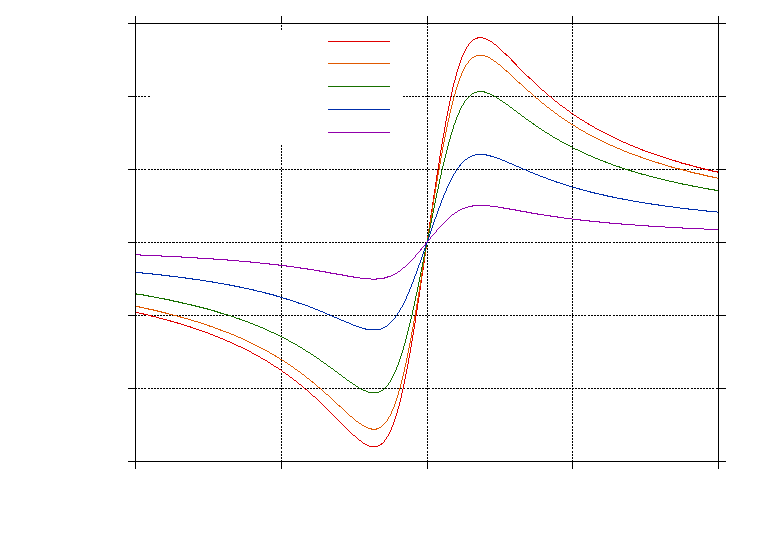
\includegraphics{Figures/Delta4/kdepend}}%
    \gplfronttext
  \end{picture}%
\endgroup
  
\caption{The numerically calculated gap $\Delta_k$ is plotted as a function of $k$ for different temperatures. Notice, that it has a maximum around $k = 1.8 k_F$. Parameters: $(n_Ba_B^3)^{1/3} = 0.01$, $(n_Ba_{BF}^3)^{1/3} = 0.1$, $l_t = 0$, $\frac{m_B}{m_F} = 7/40$, $\frac{n_F}{n_B^{1/3}} = 0.215$, $v_F/c_0 = 0.33$. }  
\label{fig.Deltakkdepend}  
\end{center}    
\end{figure}

A note on the chosen phase of $\Delta_k$. Let me therefore write $\Delta_k = \Delta_{k,0}\text{e}^{i\phi}$. In the numerical calculation we have chosen a \textit{real} function as a starting guess for $\Delta_k$. The numerical calculation then shows, that such a \textit{real} solution can be found. This amounts to \textit{choosing} a specific phase $\phi$ of $\Delta_k$, namely $\phi = 0$. Now, the mean field $\braket{\psi(x')\psi(x)}$ can be found from equation \ref{eq.correlation} to be:
\begin{equation}
\braket{\psi(x')\psi(x)} = i\int \frac{dk}{2\pi} \sin(kx)\frac{\Delta_k}{2E_{F,k}}\tanh\left[\frac{ \beta E_{F,k} }{2}\right]. \nonumber
\end{equation}
This I will show in more detail later in this chapter. By choosing the phase of $\Delta_k$, we are therefore choosing the phase of the mean field. From the gap equation it is clear, that we could have picked this phase to be whatever we like. This is what is meant, when the term "spontaneous symmetry breaking" is used. We can for any choice of the phase $\phi$ find a solution, but we \textit{have} to choose a specific one.\footnote{This is equivalent to the symmetry breaking of a spin chain. Here it is the polarization of the spins, that is chosen spontaneously, when the system is cooled.} This symmetry breaking has other important physical consequences. Those I will return to later on. 

\begin{figure} 
\begin{center}  
% GNUPLOT: LaTeX picture with Postscript
\begingroup
  \makeatletter
  \providecommand\color[2][]{%
    \GenericError{(gnuplot) \space\space\space\@spaces}{%
      Package color not loaded in conjunction with
      terminal option `colourtext'%
    }{See the gnuplot documentation for explanation.%
    }{Either use 'blacktext' in gnuplot or load the package
      color.sty in LaTeX.}%
    \renewcommand\color[2][]{}%
  }%
  \providecommand\includegraphics[2][]{%
    \GenericError{(gnuplot) \space\space\space\@spaces}{%
      Package graphicx or graphics not loaded%
    }{See the gnuplot documentation for explanation.%
    }{The gnuplot epslatex terminal needs graphicx.sty or graphics.sty.}%
    \renewcommand\includegraphics[2][]{}%
  }%
  \providecommand\rotatebox[2]{#2}%
  \@ifundefined{ifGPcolor}{%
    \newif\ifGPcolor
    \GPcolorfalse
  }{}%
  \@ifundefined{ifGPblacktext}{%
    \newif\ifGPblacktext
    \GPblacktexttrue
  }{}%
  % define a \g@addto@macro without @ in the name:
  \let\gplgaddtomacro\g@addto@macro
  % define empty templates for all commands taking text:
  \gdef\gplbacktext{}%
  \gdef\gplfronttext{}%
  \makeatother
  \ifGPblacktext
    % no textcolor at all
    \def\colorrgb#1{}%
    \def\colorgray#1{}%
  \else
    % gray or color?
    \ifGPcolor
      \def\colorrgb#1{\color[rgb]{#1}}%
      \def\colorgray#1{\color[gray]{#1}}%
      \expandafter\def\csname LTw\endcsname{\color{white}}%
      \expandafter\def\csname LTb\endcsname{\color{black}}%
      \expandafter\def\csname LTa\endcsname{\color{black}}%
      \expandafter\def\csname LT0\endcsname{\color[rgb]{1,0,0}}%
      \expandafter\def\csname LT1\endcsname{\color[rgb]{0,1,0}}%
      \expandafter\def\csname LT2\endcsname{\color[rgb]{0,0,1}}%
      \expandafter\def\csname LT3\endcsname{\color[rgb]{1,0,1}}%
      \expandafter\def\csname LT4\endcsname{\color[rgb]{0,1,1}}%
      \expandafter\def\csname LT5\endcsname{\color[rgb]{1,1,0}}%
      \expandafter\def\csname LT6\endcsname{\color[rgb]{0,0,0}}%
      \expandafter\def\csname LT7\endcsname{\color[rgb]{1,0.3,0}}%
      \expandafter\def\csname LT8\endcsname{\color[rgb]{0.5,0.5,0.5}}%
    \else
      % gray
      \def\colorrgb#1{\color{black}}%
      \def\colorgray#1{\color[gray]{#1}}%
      \expandafter\def\csname LTw\endcsname{\color{white}}%
      \expandafter\def\csname LTb\endcsname{\color{black}}%
      \expandafter\def\csname LTa\endcsname{\color{black}}%
      \expandafter\def\csname LT0\endcsname{\color{black}}%
      \expandafter\def\csname LT1\endcsname{\color{black}}%
      \expandafter\def\csname LT2\endcsname{\color{black}}%
      \expandafter\def\csname LT3\endcsname{\color{black}}%
      \expandafter\def\csname LT4\endcsname{\color{black}}%
      \expandafter\def\csname LT5\endcsname{\color{black}}%
      \expandafter\def\csname LT6\endcsname{\color{black}}%
      \expandafter\def\csname LT7\endcsname{\color{black}}%
      \expandafter\def\csname LT8\endcsname{\color{black}}%
    \fi
  \fi
    \setlength{\unitlength}{0.0500bp}%
    \ifx\gptboxheight\undefined%
      \newlength{\gptboxheight}%
      \newlength{\gptboxwidth}%
      \newsavebox{\gptboxtext}%
    \fi%
    \setlength{\fboxrule}{0.5pt}%
    \setlength{\fboxsep}{1pt}%
\begin{picture}(7200.00,5040.00)%
    \gplgaddtomacro\gplbacktext{%
      \csname LTb\endcsname%
      \put(946,767){\makebox(0,0)[r]{\strut{}$0$}}%
      \csname LTb\endcsname%
      \put(946,1469){\makebox(0,0)[r]{\strut{}$0.05$}}%
      \csname LTb\endcsname%
      \put(946,2170){\makebox(0,0)[r]{\strut{}$0.1$}}%
      \csname LTb\endcsname%
      \put(946,2872){\makebox(0,0)[r]{\strut{}$0.15$}}%
      \csname LTb\endcsname%
      \put(946,3573){\makebox(0,0)[r]{\strut{}$0.2$}}%
      \csname LTb\endcsname%
      \put(946,4275){\makebox(0,0)[r]{\strut{}$0.25$}}%
      \csname LTb\endcsname%
      \put(946,4976){\makebox(0,0)[r]{\strut{}$0.3$}}%
      \csname LTb\endcsname%
      \put(1141,484){\makebox(0,0){\strut{}$0$}}%
      \csname LTb\endcsname%
      \put(1888,484){\makebox(0,0){\strut{}$0.02$}}%
      \csname LTb\endcsname%
      \put(2634,484){\makebox(0,0){\strut{}$0.04$}}%
      \csname LTb\endcsname%
      \put(3381,484){\makebox(0,0){\strut{}$0.06$}}%
      \csname LTb\endcsname%
      \put(4127,484){\makebox(0,0){\strut{}$0.08$}}%
      \csname LTb\endcsname%
      \put(4874,484){\makebox(0,0){\strut{}$0.1$}}%
      \csname LTb\endcsname%
      \put(5620,484){\makebox(0,0){\strut{}$0.12$}}%
      \csname LTb\endcsname%
      \put(6367,484){\makebox(0,0){\strut{}$0.14$}}%
    }%
    \gplgaddtomacro\gplfronttext{%
      \csname LTb\endcsname%
      \put(176,2871){\rotatebox{-270}{\makebox(0,0){\strut{}$\max_k[\Delta_k]/\epsilon_{F,0}$}}}%
      \put(3940,154){\makebox(0,0){\strut{}$T/T_F$}}%
    }%
    \gplbacktext
    \put(0,0){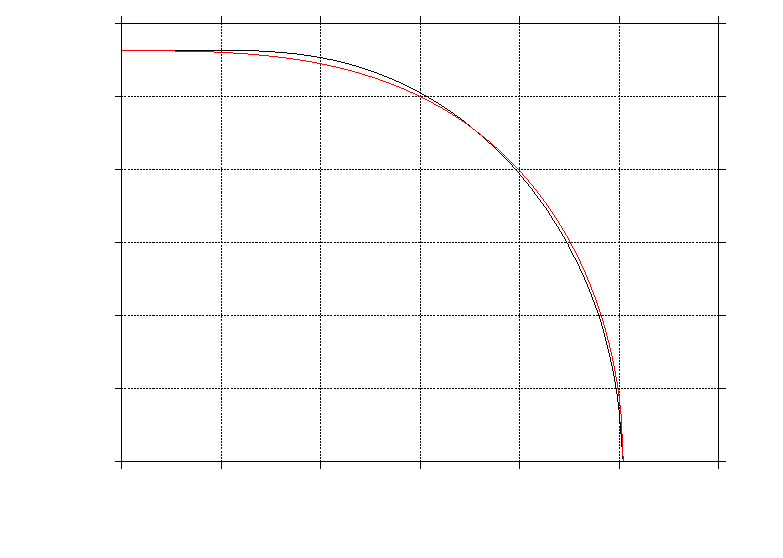
\includegraphics{Figures/Delta4/Tdepend}}%
    \gplfronttext
  \end{picture}%
\endgroup
  
\caption{In black: The numerically calculated maximal pairing $\max_k[\Delta_k]$. In red: the asymptotic form from equation \eqref{eq.maxpairingasymp}. This is seen to fit very well for both $T/T_c \ll 1$ and $T/T_c \approx 1$. Notice, that the critical temperature at which the pairing vanishes is $T_c \approx 0.129 T_F$, and that the gap is rapidly decreasing in the region $0.08< T/T_F < 0.129$. Parameters: $(n_Ba_B^3)^{1/3} = 0.01$, $(n_Ba_{BF}^3)^{1/3} = 0.1$, $l_t = 0$, $\frac{m_B}{m_F} = 7/40$, $\frac{n_F}{n_B^{1/3}} = 0.215$, $v_F/c_0 = 0.33$. }  
\label{fig.maxkDeltakTdepend}  
\end{center}    
\end{figure}

We observe for the solution at hand, that the pairing potential is uneven in $k$ as already argued, and that it goes to 0 for $k/k_F \gg 1$. This decay does not seem to be exponential, but rather of a power type. Further, the maximum value of the gap $\max_k[\Delta_k]$ decreases monotonically to 0 in a similar manner to the original BCS-theory. See \cite{Tinkham,BruusFlensberg,PlischkeStatPhys} for details. Finally, the chemical potential has not been plotted. Since the chemical potential numerically changes very little from the free gas potential, a very high resolution in $k$ is needed to get an accurate numerical result. Therefore, we do not plot the chemical potential and instead use the number equation only to enhance the precision of the found pairing. We do however see, that the chemical potential is shifted downwards for $T = 0$. This is physically reasonable, since it should cost less energy to add another fermion, when they are (partially) attracting each other through the induced interaction. Further, since the pairing goes continously to zero for $T\to T_c$ the chemical potential must go continuously to the free gas potential for $T\to T_c$. 


\subsection{The relevant momenta and the coupling potential}
In this subsection we will see how the energy dispersion and the mean occupancy of the $k$'th state behave in an extreme case for the relative densities of the Bose and Fermi gases. This will explain, why it is momenta around the Fermi momentum ($k \approx k_F$), that are relevant to understand the influence of the pairing. 

In figures \ref{fig.EnergyDispersion} and \ref{fig.Occupancy} we have plotted the energy dispersion $E_{F,k}$ and occupancy $\braket{f_k^\dagger f_k}$ for $T = 0$ for different values of the Bose gas parameter $r_B = (n_Ba_B^3)^{1/3}$. Firstly, the energy dispersion plot show, in particular for the red line, that the main difference relative to the free gas dispersion, in black, is to be found around the Fermi momentum $k_F$. If one had plotted out to the value of $k$, where the pairing has its maximum, $k_{\max} \approx 13 k_F$ in the present case, we would see, that the energy dispersion is hardly altered at all by the pairing. This is also clear from the functional form: $E_{F,k}/\epsilon_{F,0} = [(k^2/k_F^2 - \mu(0)/\epsilon_{F,0})^2 + |\Delta_k/\epsilon_{F,0}|^2 ]^{1/2}$; the first term $(k^2/k_F^2 - \mu(0)/\epsilon_{F,0})^2$ quickly becomes dominant for high values of $k/k_F$. Secondly, the number of fermions with momentum $k$ (the occupancy of the $k$'th state), $\braket{f_k^\dagger f_k}$, is seen to be significant only for $k < 2k_F$. Hence, even if the effect at high momenta $k \gg k_F$ of the pairing on the energy dispersion had been significant, it would have been suppressed by the fact, that there are simply no fermions moving with such high momenta.

The occupancy plot in particular shows, that the Fermi sphere is increasingly blurred out for decreasing values of $(n_Ba_B^3)^{1/3}$.\footnote{Since the string is one-dimensional, the Fermi sphere only consists of two points: $k = \pm k_F$.} 

This is done for a high value of the boson density $n_B$: $\frac{n_F}{n_B^{1/3}} = 0.0215$, since it is for these high boson densities the maximum of the pairing is moved to high values of $k/k_F$. The reason for this can be understood physically in the following way. When the density of the bosons becomes very large, the rigidity of the gas increases; it simply becomes harder to suppress the gas. Therefore, to get a significant pairing of two fermions, they need to move at a relatively high speed resulting in a pairing with a maximum at high values of $k/k_F$. This effect can be studied further by plotting the induced coupling potential $W_{FF}^{\text{ind}}(k,k')$ as a function of the relative particle distance $\frac{n_F}{n_B^{1/3}}$. With the arguments of the above, we will do this for $k = k' = k_F$. We see, that $W_{FF}^{\text{ind}}(k_F,k_F)$ has an extremal point. The behaviour for low values of $\frac{n_F}{n_B^{1/3}}$ can be understood in the same way as the above. When the density of the boson gas increases, the fermions have a harder time creating ripples in the gas, and the coupling goes down. For high values of $\frac{n_F}{n_B^{1/3}}$ on the other hand, the boson gas is depleted, $n_B$ decreases, and there are simply fewer bosons around for the fermions to interact with. This is in complete accordance with what is seen in an equivalent 2D-3D system studied in the article \cite{BruunZhigangTopSuperfluid}. 

In connection with the neglection of retardation effects we actually already used, that the typical speed of the fermions is the Fermi speed $v_F = k_F/m_F$. The present subsection therefore shows, that this assumption is selfconsistent. 

I will emphasize, that in particular the red graphs of figures \ref{fig.EnergyDispersion} and \ref{fig.Occupancy} suggest, that we are entering a strong coupling regime. The reason for this is, that we are strongly changing the statistics of the fermions. Hence, the weak coupling theory we are using is expected to break down. The point still remains: the plots show, that we have to go to extreme values of $n_B/n_F^3$, before we get into trouble with the weak coupling theory, and still here we expect, that the relevant momenta are around the Fermi momentum. 


\begin{figure} 
\begin{center}  
% GNUPLOT: LaTeX picture with Postscript
\begingroup
  \makeatletter
  \providecommand\color[2][]{%
    \GenericError{(gnuplot) \space\space\space\@spaces}{%
      Package color not loaded in conjunction with
      terminal option `colourtext'%
    }{See the gnuplot documentation for explanation.%
    }{Either use 'blacktext' in gnuplot or load the package
      color.sty in LaTeX.}%
    \renewcommand\color[2][]{}%
  }%
  \providecommand\includegraphics[2][]{%
    \GenericError{(gnuplot) \space\space\space\@spaces}{%
      Package graphicx or graphics not loaded%
    }{See the gnuplot documentation for explanation.%
    }{The gnuplot epslatex terminal needs graphicx.sty or graphics.sty.}%
    \renewcommand\includegraphics[2][]{}%
  }%
  \providecommand\rotatebox[2]{#2}%
  \@ifundefined{ifGPcolor}{%
    \newif\ifGPcolor
    \GPcolortrue
  }{}%
  \@ifundefined{ifGPblacktext}{%
    \newif\ifGPblacktext
    \GPblacktexttrue
  }{}%
  % define a \g@addto@macro without @ in the name:
  \let\gplgaddtomacro\g@addto@macro
  % define empty templates for all commands taking text:
  \gdef\gplbacktext{}%
  \gdef\gplfronttext{}%
  \makeatother
  \ifGPblacktext
    % no textcolor at all
    \def\colorrgb#1{}%
    \def\colorgray#1{}%
  \else
    % gray or color?
    \ifGPcolor
      \def\colorrgb#1{\color[rgb]{#1}}%
      \def\colorgray#1{\color[gray]{#1}}%
      \expandafter\def\csname LTw\endcsname{\color{white}}%
      \expandafter\def\csname LTb\endcsname{\color{black}}%
      \expandafter\def\csname LTa\endcsname{\color{black}}%
      \expandafter\def\csname LT0\endcsname{\color[rgb]{1,0,0}}%
      \expandafter\def\csname LT1\endcsname{\color[rgb]{0,1,0}}%
      \expandafter\def\csname LT2\endcsname{\color[rgb]{0,0,1}}%
      \expandafter\def\csname LT3\endcsname{\color[rgb]{1,0,1}}%
      \expandafter\def\csname LT4\endcsname{\color[rgb]{0,1,1}}%
      \expandafter\def\csname LT5\endcsname{\color[rgb]{1,1,0}}%
      \expandafter\def\csname LT6\endcsname{\color[rgb]{0,0,0}}%
      \expandafter\def\csname LT7\endcsname{\color[rgb]{1,0.3,0}}%
      \expandafter\def\csname LT8\endcsname{\color[rgb]{0.5,0.5,0.5}}%
    \else
      % gray
      \def\colorrgb#1{\color{black}}%
      \def\colorgray#1{\color[gray]{#1}}%
      \expandafter\def\csname LTw\endcsname{\color{white}}%
      \expandafter\def\csname LTb\endcsname{\color{black}}%
      \expandafter\def\csname LTa\endcsname{\color{black}}%
      \expandafter\def\csname LT0\endcsname{\color{black}}%
      \expandafter\def\csname LT1\endcsname{\color{black}}%
      \expandafter\def\csname LT2\endcsname{\color{black}}%
      \expandafter\def\csname LT3\endcsname{\color{black}}%
      \expandafter\def\csname LT4\endcsname{\color{black}}%
      \expandafter\def\csname LT5\endcsname{\color{black}}%
      \expandafter\def\csname LT6\endcsname{\color{black}}%
      \expandafter\def\csname LT7\endcsname{\color{black}}%
      \expandafter\def\csname LT8\endcsname{\color{black}}%
    \fi
  \fi
    \setlength{\unitlength}{0.0500bp}%
    \ifx\gptboxheight\undefined%
      \newlength{\gptboxheight}%
      \newlength{\gptboxwidth}%
      \newsavebox{\gptboxtext}%
    \fi%
    \setlength{\fboxrule}{0.5pt}%
    \setlength{\fboxsep}{1pt}%
\begin{picture}(7200.00,5040.00)%
    \gplgaddtomacro\gplbacktext{%
      \csname LTb\endcsname%
      \put(682,767){\makebox(0,0)[r]{\strut{}$0$}}%
      \csname LTb\endcsname%
      \put(682,1609){\makebox(0,0)[r]{\strut{}$2$}}%
      \csname LTb\endcsname%
      \put(682,2451){\makebox(0,0)[r]{\strut{}$4$}}%
      \csname LTb\endcsname%
      \put(682,3292){\makebox(0,0)[r]{\strut{}$6$}}%
      \csname LTb\endcsname%
      \put(682,4134){\makebox(0,0)[r]{\strut{}$8$}}%
      \csname LTb\endcsname%
      \put(682,4976){\makebox(0,0)[r]{\strut{}$10$}}%
      \csname LTb\endcsname%
      \put(877,484){\makebox(0,0){\strut{}$0$}}%
      \csname LTb\endcsname%
      \put(1854,484){\makebox(0,0){\strut{}$0.5$}}%
      \csname LTb\endcsname%
      \put(2831,484){\makebox(0,0){\strut{}$1$}}%
      \csname LTb\endcsname%
      \put(3809,484){\makebox(0,0){\strut{}$1.5$}}%
      \csname LTb\endcsname%
      \put(4786,484){\makebox(0,0){\strut{}$2$}}%
      \csname LTb\endcsname%
      \put(5763,484){\makebox(0,0){\strut{}$2.5$}}%
      \csname LTb\endcsname%
      \put(6740,484){\makebox(0,0){\strut{}$3$}}%
    }%
    \gplgaddtomacro\gplfronttext{%
      \csname LTb\endcsname%
      \put(176,2871){\rotatebox{-270}{\makebox(0,0){\strut{}$ E_{F,k}$}}}%
      \put(3808,154){\makebox(0,0){\strut{}$k/k_F$}}%
      \csname LTb\endcsname%
      \put(2329,4803){\makebox(0,0)[r]{\strut{}Free gas}}%
      \csname LTb\endcsname%
      \put(2329,4583){\makebox(0,0)[r]{\strut{}$r_B = 0.005$}}%
      \csname LTb\endcsname%
      \put(2329,4363){\makebox(0,0)[r]{\strut{}$r_B = 0.006$}}%
      \csname LTb\endcsname%
      \put(2329,4143){\makebox(0,0)[r]{\strut{}$r_B = 0.007$}}%
      \csname LTb\endcsname%
      \put(2329,3923){\makebox(0,0)[r]{\strut{}$r_B = 0.010$}}%
    }%
    \gplbacktext
    \put(0,0){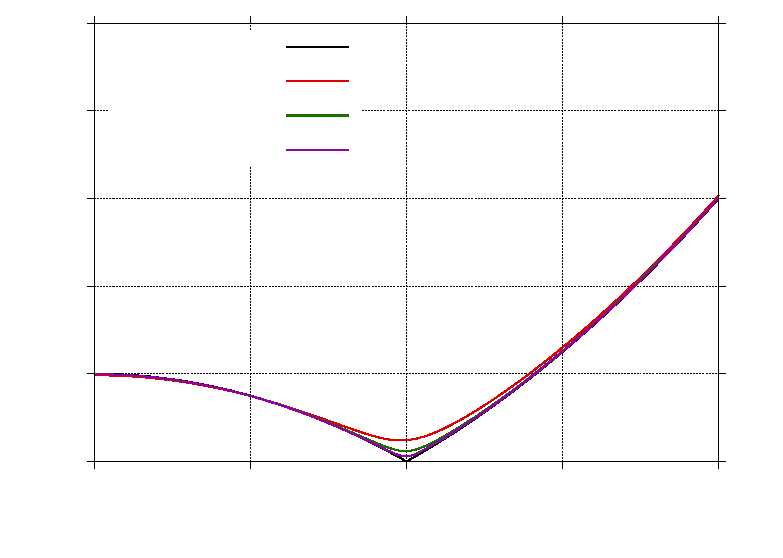
\includegraphics{energyplot}}%
    \gplfronttext
  \end{picture}%
\endgroup
  
\caption{The energy dispersion is plotted for $T = 0$. Coloured lines: differing values of the Bose gas parameter $r_B = (n_Ba_B^3)^{1/3}$, superconductiong phase. Black line: free gas (normal phase) energy dispersion. The energy is even in $k$, so the graphs are just mirrored for $k < 0$. Other parameters: $(n_Ba_{BF}^3)^{1/3} = 0.1, \frac{m_B}{m_F} = 7/40, \frac{n_F}{n_B^{1/3}} = 0.0215.$ }  
\label{fig.EnergyDispersion}  
\end{center}    
\end{figure}


\begin{figure} 
\begin{center}  
% GNUPLOT: LaTeX picture with Postscript
\begingroup
  \makeatletter
  \providecommand\color[2][]{%
    \GenericError{(gnuplot) \space\space\space\@spaces}{%
      Package color not loaded in conjunction with
      terminal option `colourtext'%
    }{See the gnuplot documentation for explanation.%
    }{Either use 'blacktext' in gnuplot or load the package
      color.sty in LaTeX.}%
    \renewcommand\color[2][]{}%
  }%
  \providecommand\includegraphics[2][]{%
    \GenericError{(gnuplot) \space\space\space\@spaces}{%
      Package graphicx or graphics not loaded%
    }{See the gnuplot documentation for explanation.%
    }{The gnuplot epslatex terminal needs graphicx.sty or graphics.sty.}%
    \renewcommand\includegraphics[2][]{}%
  }%
  \providecommand\rotatebox[2]{#2}%
  \@ifundefined{ifGPcolor}{%
    \newif\ifGPcolor
    \GPcolortrue
  }{}%
  \@ifundefined{ifGPblacktext}{%
    \newif\ifGPblacktext
    \GPblacktexttrue
  }{}%
  % define a \g@addto@macro without @ in the name:
  \let\gplgaddtomacro\g@addto@macro
  % define empty templates for all commands taking text:
  \gdef\gplbacktext{}%
  \gdef\gplfronttext{}%
  \makeatother
  \ifGPblacktext
    % no textcolor at all
    \def\colorrgb#1{}%
    \def\colorgray#1{}%
  \else
    % gray or color?
    \ifGPcolor
      \def\colorrgb#1{\color[rgb]{#1}}%
      \def\colorgray#1{\color[gray]{#1}}%
      \expandafter\def\csname LTw\endcsname{\color{white}}%
      \expandafter\def\csname LTb\endcsname{\color{black}}%
      \expandafter\def\csname LTa\endcsname{\color{black}}%
      \expandafter\def\csname LT0\endcsname{\color[rgb]{1,0,0}}%
      \expandafter\def\csname LT1\endcsname{\color[rgb]{0,1,0}}%
      \expandafter\def\csname LT2\endcsname{\color[rgb]{0,0,1}}%
      \expandafter\def\csname LT3\endcsname{\color[rgb]{1,0,1}}%
      \expandafter\def\csname LT4\endcsname{\color[rgb]{0,1,1}}%
      \expandafter\def\csname LT5\endcsname{\color[rgb]{1,1,0}}%
      \expandafter\def\csname LT6\endcsname{\color[rgb]{0,0,0}}%
      \expandafter\def\csname LT7\endcsname{\color[rgb]{1,0.3,0}}%
      \expandafter\def\csname LT8\endcsname{\color[rgb]{0.5,0.5,0.5}}%
    \else
      % gray
      \def\colorrgb#1{\color{black}}%
      \def\colorgray#1{\color[gray]{#1}}%
      \expandafter\def\csname LTw\endcsname{\color{white}}%
      \expandafter\def\csname LTb\endcsname{\color{black}}%
      \expandafter\def\csname LTa\endcsname{\color{black}}%
      \expandafter\def\csname LT0\endcsname{\color{black}}%
      \expandafter\def\csname LT1\endcsname{\color{black}}%
      \expandafter\def\csname LT2\endcsname{\color{black}}%
      \expandafter\def\csname LT3\endcsname{\color{black}}%
      \expandafter\def\csname LT4\endcsname{\color{black}}%
      \expandafter\def\csname LT5\endcsname{\color{black}}%
      \expandafter\def\csname LT6\endcsname{\color{black}}%
      \expandafter\def\csname LT7\endcsname{\color{black}}%
      \expandafter\def\csname LT8\endcsname{\color{black}}%
    \fi
  \fi
    \setlength{\unitlength}{0.0500bp}%
    \ifx\gptboxheight\undefined%
      \newlength{\gptboxheight}%
      \newlength{\gptboxwidth}%
      \newsavebox{\gptboxtext}%
    \fi%
    \setlength{\fboxrule}{0.5pt}%
    \setlength{\fboxsep}{1pt}%
\begin{picture}(7200.00,5040.00)%
    \gplgaddtomacro\gplbacktext{%
      \csname LTb\endcsname%
      \put(814,767){\makebox(0,0)[r]{\strut{}$0$}}%
      \csname LTb\endcsname%
      \put(814,1532){\makebox(0,0)[r]{\strut{}$0.2$}}%
      \csname LTb\endcsname%
      \put(814,2298){\makebox(0,0)[r]{\strut{}$0.4$}}%
      \csname LTb\endcsname%
      \put(814,3063){\makebox(0,0)[r]{\strut{}$0.6$}}%
      \csname LTb\endcsname%
      \put(814,3828){\makebox(0,0)[r]{\strut{}$0.8$}}%
      \csname LTb\endcsname%
      \put(814,4593){\makebox(0,0)[r]{\strut{}$1$}}%
      \csname LTb\endcsname%
      \put(1009,484){\makebox(0,0){\strut{}$0$}}%
      \csname LTb\endcsname%
      \put(2442,484){\makebox(0,0){\strut{}$0.5$}}%
      \csname LTb\endcsname%
      \put(3875,484){\makebox(0,0){\strut{}$1$}}%
      \csname LTb\endcsname%
      \put(5307,484){\makebox(0,0){\strut{}$1.5$}}%
      \csname LTb\endcsname%
      \put(6740,484){\makebox(0,0){\strut{}$2$}}%
    }%
    \gplgaddtomacro\gplfronttext{%
      \csname LTb\endcsname%
      \put(176,2871){\rotatebox{-270}{\makebox(0,0){\strut{}$\braket{c_k^\dagger c_k}$}}}%
      \put(3874,154){\makebox(0,0){\strut{}$k/k_F$}}%
      \csname LTb\endcsname%
      \put(5753,4803){\makebox(0,0)[r]{\strut{}Free gas}}%
      \csname LTb\endcsname%
      \put(5753,4583){\makebox(0,0)[r]{\strut{}$r_B = 0.005$}}%
      \csname LTb\endcsname%
      \put(5753,4363){\makebox(0,0)[r]{\strut{}$r_B = 0.006$}}%
      \csname LTb\endcsname%
      \put(5753,4143){\makebox(0,0)[r]{\strut{}$r_B = 0.007$}}%
      \csname LTb\endcsname%
      \put(5753,3923){\makebox(0,0)[r]{\strut{}$r_B = 0.010$}}%
    }%
    \gplbacktext
    \put(0,0){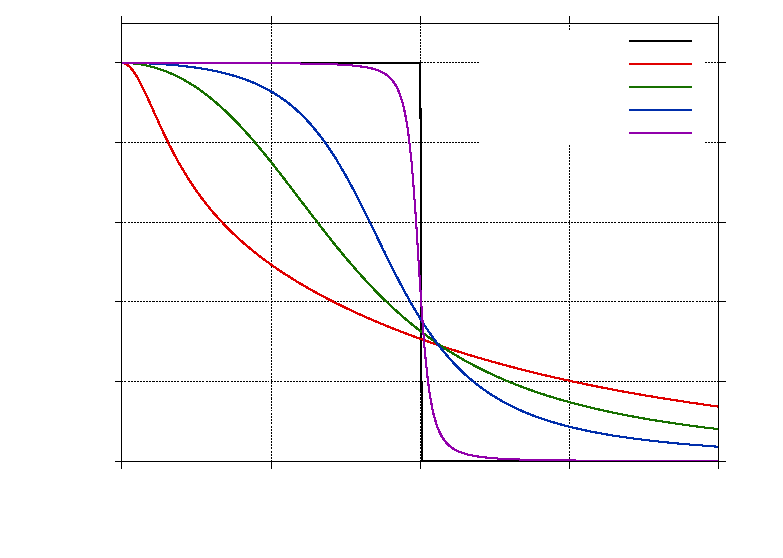
\includegraphics{Figures/OccupancyT0/Occupancyplot}}%
    \gplfronttext
  \end{picture}%
\endgroup
  
\caption{The number of fermions with momentum $k$, $\braket{f_k^\dagger f_k}$, is plotted for $T = 0$. $\braket{f_k^\dagger f_k} = |v_{F,k}|^2 = \frac{1}{2}\left(1 - \frac{\epsilon_k}{E_{F,k}}\right)$. Coloured lines: differing values of the Bose gas parameter $r_B = (n_Ba_B^3)^{1/3}$, superfluid phase. Black line: Fermi-Dirac distribution for the free gas (normal phase).  Other parameters: $(n_Ba_{BF}^3)^{1/3} = 0.1, \frac{m_B}{m_F} = 7/40, \frac{n_F}{n_B^{1/3}} = 0.0215.$  }  
\label{fig.Occupancy}  
\end{center}    
\end{figure}

\begin{figure} 
\begin{center}  
% GNUPLOT: LaTeX picture with Postscript
\begingroup
  \makeatletter
  \providecommand\color[2][]{%
    \GenericError{(gnuplot) \space\space\space\@spaces}{%
      Package color not loaded in conjunction with
      terminal option `colourtext'%
    }{See the gnuplot documentation for explanation.%
    }{Either use 'blacktext' in gnuplot or load the package
      color.sty in LaTeX.}%
    \renewcommand\color[2][]{}%
  }%
  \providecommand\includegraphics[2][]{%
    \GenericError{(gnuplot) \space\space\space\@spaces}{%
      Package graphicx or graphics not loaded%
    }{See the gnuplot documentation for explanation.%
    }{The gnuplot epslatex terminal needs graphicx.sty or graphics.sty.}%
    \renewcommand\includegraphics[2][]{}%
  }%
  \providecommand\rotatebox[2]{#2}%
  \@ifundefined{ifGPcolor}{%
    \newif\ifGPcolor
    \GPcolortrue
  }{}%
  \@ifundefined{ifGPblacktext}{%
    \newif\ifGPblacktext
    \GPblacktexttrue
  }{}%
  % define a \g@addto@macro without @ in the name:
  \let\gplgaddtomacro\g@addto@macro
  % define empty templates for all commands taking text:
  \gdef\gplbacktext{}%
  \gdef\gplfronttext{}%
  \makeatother
  \ifGPblacktext
    % no textcolor at all
    \def\colorrgb#1{}%
    \def\colorgray#1{}%
  \else
    % gray or color?
    \ifGPcolor
      \def\colorrgb#1{\color[rgb]{#1}}%
      \def\colorgray#1{\color[gray]{#1}}%
      \expandafter\def\csname LTw\endcsname{\color{white}}%
      \expandafter\def\csname LTb\endcsname{\color{black}}%
      \expandafter\def\csname LTa\endcsname{\color{black}}%
      \expandafter\def\csname LT0\endcsname{\color[rgb]{1,0,0}}%
      \expandafter\def\csname LT1\endcsname{\color[rgb]{0,1,0}}%
      \expandafter\def\csname LT2\endcsname{\color[rgb]{0,0,1}}%
      \expandafter\def\csname LT3\endcsname{\color[rgb]{1,0,1}}%
      \expandafter\def\csname LT4\endcsname{\color[rgb]{0,1,1}}%
      \expandafter\def\csname LT5\endcsname{\color[rgb]{1,1,0}}%
      \expandafter\def\csname LT6\endcsname{\color[rgb]{0,0,0}}%
      \expandafter\def\csname LT7\endcsname{\color[rgb]{1,0.3,0}}%
      \expandafter\def\csname LT8\endcsname{\color[rgb]{0.5,0.5,0.5}}%
    \else
      % gray
      \def\colorrgb#1{\color{black}}%
      \def\colorgray#1{\color[gray]{#1}}%
      \expandafter\def\csname LTw\endcsname{\color{white}}%
      \expandafter\def\csname LTb\endcsname{\color{black}}%
      \expandafter\def\csname LTa\endcsname{\color{black}}%
      \expandafter\def\csname LT0\endcsname{\color{black}}%
      \expandafter\def\csname LT1\endcsname{\color{black}}%
      \expandafter\def\csname LT2\endcsname{\color{black}}%
      \expandafter\def\csname LT3\endcsname{\color{black}}%
      \expandafter\def\csname LT4\endcsname{\color{black}}%
      \expandafter\def\csname LT5\endcsname{\color{black}}%
      \expandafter\def\csname LT6\endcsname{\color{black}}%
      \expandafter\def\csname LT7\endcsname{\color{black}}%
      \expandafter\def\csname LT8\endcsname{\color{black}}%
    \fi
  \fi
    \setlength{\unitlength}{0.0500bp}%
    \ifx\gptboxheight\undefined%
      \newlength{\gptboxheight}%
      \newlength{\gptboxwidth}%
      \newsavebox{\gptboxtext}%
    \fi%
    \setlength{\fboxrule}{0.5pt}%
    \setlength{\fboxsep}{1pt}%
\begin{picture}(7200.00,5040.00)%
    \gplgaddtomacro\gplbacktext{%
      \csname LTb\endcsname%
      \put(946,767){\makebox(0,0)[r]{\strut{}$-2.5$}}%
      \csname LTb\endcsname%
      \put(946,1609){\makebox(0,0)[r]{\strut{}$-2$}}%
      \csname LTb\endcsname%
      \put(946,2451){\makebox(0,0)[r]{\strut{}$-1.5$}}%
      \csname LTb\endcsname%
      \put(946,3292){\makebox(0,0)[r]{\strut{}$-1$}}%
      \csname LTb\endcsname%
      \put(946,4134){\makebox(0,0)[r]{\strut{}$-0.5$}}%
      \csname LTb\endcsname%
      \put(946,4976){\makebox(0,0)[r]{\strut{}$0$}}%
      \csname LTb\endcsname%
      \put(1141,484){\makebox(0,0){\strut{}$0$}}%
      \csname LTb\endcsname%
      \put(1841,484){\makebox(0,0){\strut{}$0.1$}}%
      \csname LTb\endcsname%
      \put(2541,484){\makebox(0,0){\strut{}$0.2$}}%
      \csname LTb\endcsname%
      \put(3241,484){\makebox(0,0){\strut{}$0.3$}}%
      \csname LTb\endcsname%
      \put(3941,484){\makebox(0,0){\strut{}$0.4$}}%
      \csname LTb\endcsname%
      \put(4640,484){\makebox(0,0){\strut{}$0.5$}}%
      \csname LTb\endcsname%
      \put(5340,484){\makebox(0,0){\strut{}$0.6$}}%
      \csname LTb\endcsname%
      \put(6040,484){\makebox(0,0){\strut{}$0.7$}}%
      \csname LTb\endcsname%
      \put(6740,484){\makebox(0,0){\strut{}$0.8$}}%
    }%
    \gplgaddtomacro\gplfronttext{%
      \csname LTb\endcsname%
      \put(176,2871){\rotatebox{-270}{\makebox(0,0){\strut{}$2m_F/k_F W_{\text{ind}}(k_F, k_F)$}}}%
      \put(3940,154){\makebox(0,0){\strut{}$n_F^{1/3}/n_B$}}%
    }%
    \gplbacktext
    \put(0,0){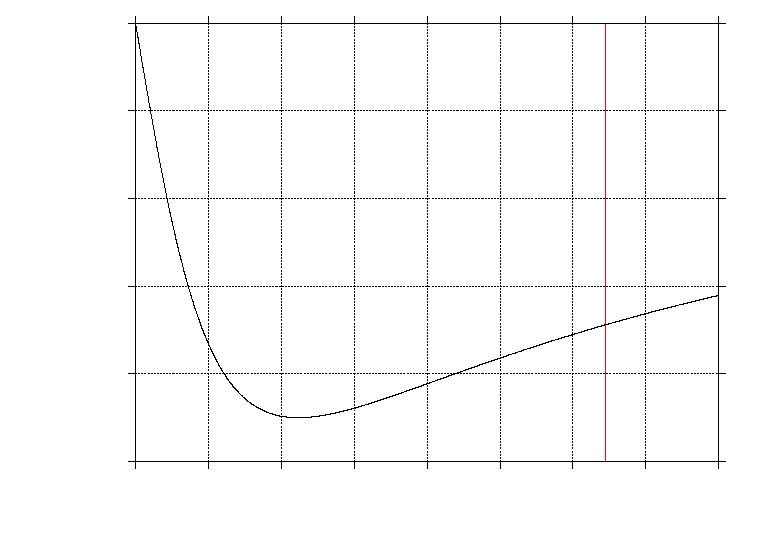
\includegraphics{Figures/InducedInteraction/InducedInteraction}}%
    \gplfronttext
  \end{picture}%
\endgroup
  
\caption{In black: The coupling potential at the Fermi surface, $W_{FF}^\text{ind}(k_F,k_F)$, as a function of relative particle distance $n_F/n_B^{1/3}$. In red: indicates where the retardation effects are expected to kick in; the line is made by requiring $v_F/c_0 < 1$. To the right of the red line the plotted potential can only be viewed as the zero frequency contribution. We notice, that the coupling potential has an extremal value. Other parameters: $(n_Ba_B^3)^{1/3} = 0.01, (n_Ba_{BF}^3)^{1/3} = 0.1, \frac{m_B}{m_F} = 7/40.$}  
\label{fig.maxkDeltakaBdepend}  
\end{center}    
\end{figure}

The fact that the maximum of the pairing can be at very high momenta means, that to figure out the functional dependency on the parameters of the system, it is much more relevant to study the behaviour of the critical temperature $T_c$ rather than the maximal pairing.\footnote{Alternatively one could study the pairing around the Fermi surface.} This will be done in chapter \ref{Chapter6}.

\subsection{The pair wave function in real space}
In this subsection we calculate the pair wave function $\braket{\psi_F(x')\psi_F(x)}$. This is a correlation function, that describes how two fermions are correlated as a function of there respective positions. Specifically a high numerical (positive or negative) value of $\braket{\psi_F(x')\psi_F(x)}$ for specific $x$ and $x'$ means, that the fermions have a tendency to be at those positions $x$ and $x'$. This is the reason why, we refer to it as the pair wave function. However, caution should be taken, since the correlation function is not a direct measure of probability. 

We have actually already calculated an unaveraged expression for the pair wave function utilizing the Fourier decomposition $\psi_F(x) = \frac{1}{\sqrt{\mathcal{L}}} \sum_k \text{e}^{ikx} f_k$ in equation \eqref{eq.correlation}. From this expression it is also clear, that it only depends on the difference $x-x'$. Therefore, we let $x \to 0, x' \to x$ in \eqref{eq.correlation}, and we obtain:
\begin{equation}
\braket{\hat{\psi}_F(x) \hat{\psi}_F(0)} = \frac{i}{\mathcal{L}}\sum_{k} \sin(kx)\braket{f_{k}f_{-k}}. \nonumber
\end{equation}
The average $\braket{f_{k}f_{-k}}$ was further calculated, when we derived the gap equation. This yielded: $\braket{f_{k}f_{-k}} = \frac{\Delta_k}{2E_{F,k}}\tanh\left[\frac{\beta E_{F,k} }{2}\right]$. Inserting this into the above and changing the sum to an integral yields:
\begin{equation}
\braket{\hat{\psi}_F(x) \hat{\psi}_F(0)} = i\int \frac{dk}{2\pi} \sin(kx)\frac{\Delta_k}{2E_{F,k}}\tanh\left[\frac{ \beta E_{F,k} }{2}\right].
\label{eq.pairwavefunction}
\end{equation}
With the pairing potential $\Delta_k$ at hand we can therefore readily calculate this function numerically. We will restrict ourselves to the $T = 0$ case, since the behaviour for $T > 0$ is quite obvious. For $T > 0$ the integrand is damped by the factor $\tanh\left[\frac{ \beta E_{F,k} }{2}\right]$, since it will be less than its maximal value of 1 for $T = 0$. Hence the correlation function will be more and more significantly damped until we reach the critical temperature $T_c$, where the pairing will vanish: $\Delta_k = 0$ as already seen. And so the correlation will also vanish for $T\to T_c$ and we regain the vanishing correlation for the free gas. Further we can see, what the overall functional behaviour must be. Firstly, we notice that the correlation function is odd in $x$, and so vanishes for $x = 0$. This is in perfect harmony with the Pauli exclusion principle: the identical fermions cannot be at the same point in space. We notice that for high values of $x$ the sine function will start to oscillate rapidly leading to rapid cancelation of the integral. Hence, we expect the correlation function to go rapidly to zero for high values of $k_F x$. 

A numerical solution is shown in figure \ref{fig.pairwavefunction}. We notice, that it is sharply peaked for $|x| \approx 1/k_F$ and so once again we have confirmed, that the length scale of the fermion-fermion distances is set by $1/k_F$. The figure here corresponds to the red graph in figure \ref{fig.Deltakkdepend}. The overall behaviour predicted above is observed. %Further, the pair wave function is seen to be a damped oscillation. The peaks do not come with a fixed period, but have an approximate distance of $k_Fx = 3.3$%

\begin{figure} 
\begin{center}  
% GNUPLOT: LaTeX picture with Postscript
\begingroup
  \makeatletter
  \providecommand\color[2][]{%
    \GenericError{(gnuplot) \space\space\space\@spaces}{%
      Package color not loaded in conjunction with
      terminal option `colourtext'%
    }{See the gnuplot documentation for explanation.%
    }{Either use 'blacktext' in gnuplot or load the package
      color.sty in LaTeX.}%
    \renewcommand\color[2][]{}%
  }%
  \providecommand\includegraphics[2][]{%
    \GenericError{(gnuplot) \space\space\space\@spaces}{%
      Package graphicx or graphics not loaded%
    }{See the gnuplot documentation for explanation.%
    }{The gnuplot epslatex terminal needs graphicx.sty or graphics.sty.}%
    \renewcommand\includegraphics[2][]{}%
  }%
  \providecommand\rotatebox[2]{#2}%
  \@ifundefined{ifGPcolor}{%
    \newif\ifGPcolor
    \GPcolorfalse
  }{}%
  \@ifundefined{ifGPblacktext}{%
    \newif\ifGPblacktext
    \GPblacktexttrue
  }{}%
  % define a \g@addto@macro without @ in the name:
  \let\gplgaddtomacro\g@addto@macro
  % define empty templates for all commands taking text:
  \gdef\gplbacktext{}%
  \gdef\gplfronttext{}%
  \makeatother
  \ifGPblacktext
    % no textcolor at all
    \def\colorrgb#1{}%
    \def\colorgray#1{}%
  \else
    % gray or color?
    \ifGPcolor
      \def\colorrgb#1{\color[rgb]{#1}}%
      \def\colorgray#1{\color[gray]{#1}}%
      \expandafter\def\csname LTw\endcsname{\color{white}}%
      \expandafter\def\csname LTb\endcsname{\color{black}}%
      \expandafter\def\csname LTa\endcsname{\color{black}}%
      \expandafter\def\csname LT0\endcsname{\color[rgb]{1,0,0}}%
      \expandafter\def\csname LT1\endcsname{\color[rgb]{0,1,0}}%
      \expandafter\def\csname LT2\endcsname{\color[rgb]{0,0,1}}%
      \expandafter\def\csname LT3\endcsname{\color[rgb]{1,0,1}}%
      \expandafter\def\csname LT4\endcsname{\color[rgb]{0,1,1}}%
      \expandafter\def\csname LT5\endcsname{\color[rgb]{1,1,0}}%
      \expandafter\def\csname LT6\endcsname{\color[rgb]{0,0,0}}%
      \expandafter\def\csname LT7\endcsname{\color[rgb]{1,0.3,0}}%
      \expandafter\def\csname LT8\endcsname{\color[rgb]{0.5,0.5,0.5}}%
    \else
      % gray
      \def\colorrgb#1{\color{black}}%
      \def\colorgray#1{\color[gray]{#1}}%
      \expandafter\def\csname LTw\endcsname{\color{white}}%
      \expandafter\def\csname LTb\endcsname{\color{black}}%
      \expandafter\def\csname LTa\endcsname{\color{black}}%
      \expandafter\def\csname LT0\endcsname{\color{black}}%
      \expandafter\def\csname LT1\endcsname{\color{black}}%
      \expandafter\def\csname LT2\endcsname{\color{black}}%
      \expandafter\def\csname LT3\endcsname{\color{black}}%
      \expandafter\def\csname LT4\endcsname{\color{black}}%
      \expandafter\def\csname LT5\endcsname{\color{black}}%
      \expandafter\def\csname LT6\endcsname{\color{black}}%
      \expandafter\def\csname LT7\endcsname{\color{black}}%
      \expandafter\def\csname LT8\endcsname{\color{black}}%
    \fi
  \fi
    \setlength{\unitlength}{0.0500bp}%
    \ifx\gptboxheight\undefined%
      \newlength{\gptboxheight}%
      \newlength{\gptboxwidth}%
      \newsavebox{\gptboxtext}%
    \fi%
    \setlength{\fboxrule}{0.5pt}%
    \setlength{\fboxsep}{1pt}%
\begin{picture}(7200.00,5040.00)%
    \gplgaddtomacro\gplbacktext{%
      \csname LTb\endcsname%
      \put(1078,767){\makebox(0,0)[r]{\strut{}$-0.1$}}%
      \csname LTb\endcsname%
      \put(1078,1819){\makebox(0,0)[r]{\strut{}$-0.05$}}%
      \csname LTb\endcsname%
      \put(1078,2872){\makebox(0,0)[r]{\strut{}$0$}}%
      \csname LTb\endcsname%
      \put(1078,3924){\makebox(0,0)[r]{\strut{}$0.05$}}%
      \csname LTb\endcsname%
      \put(1078,4976){\makebox(0,0)[r]{\strut{}$0.1$}}%
      \csname LTb\endcsname%
      \put(1273,484){\makebox(0,0){\strut{}$-20$}}%
      \csname LTb\endcsname%
      \put(1956,484){\makebox(0,0){\strut{}$-15$}}%
      \csname LTb\endcsname%
      \put(2640,484){\makebox(0,0){\strut{}$-10$}}%
      \csname LTb\endcsname%
      \put(3323,484){\makebox(0,0){\strut{}$-5$}}%
      \csname LTb\endcsname%
      \put(4007,484){\makebox(0,0){\strut{}$0$}}%
      \csname LTb\endcsname%
      \put(4690,484){\makebox(0,0){\strut{}$5$}}%
      \csname LTb\endcsname%
      \put(5373,484){\makebox(0,0){\strut{}$10$}}%
      \csname LTb\endcsname%
      \put(6057,484){\makebox(0,0){\strut{}$15$}}%
      \csname LTb\endcsname%
      \put(6740,484){\makebox(0,0){\strut{}$20$}}%
    }%
    \gplgaddtomacro\gplfronttext{%
      \csname LTb\endcsname%
      \put(176,2871){\rotatebox{-270}{\makebox(0,0){\strut{}$\braket{\psi_F(x)\psi_F(0)}/k_F $}}}%
      \put(4006,154){\makebox(0,0){\strut{}$k_Fx$}}%
      \csname LTb\endcsname%
      \put(5753,4803){\makebox(0,0)[r]{\strut{}$T/T_F = 0.000$}}%
      \csname LTb\endcsname%
      \put(5753,4583){\makebox(0,0)[r]{\strut{}$T/T_F = 0.075$}}%
      \csname LTb\endcsname%
      \put(5753,4363){\makebox(0,0)[r]{\strut{}$T/T_F = 0.100$}}%
      \csname LTb\endcsname%
      \put(5753,4143){\makebox(0,0)[r]{\strut{}$T/T_F = 0.120$}}%
      \csname LTb\endcsname%
      \put(5753,3923){\makebox(0,0)[r]{\strut{}$T/T_F = 0.127$}}%
    }%
    \gplbacktext
    \put(0,0){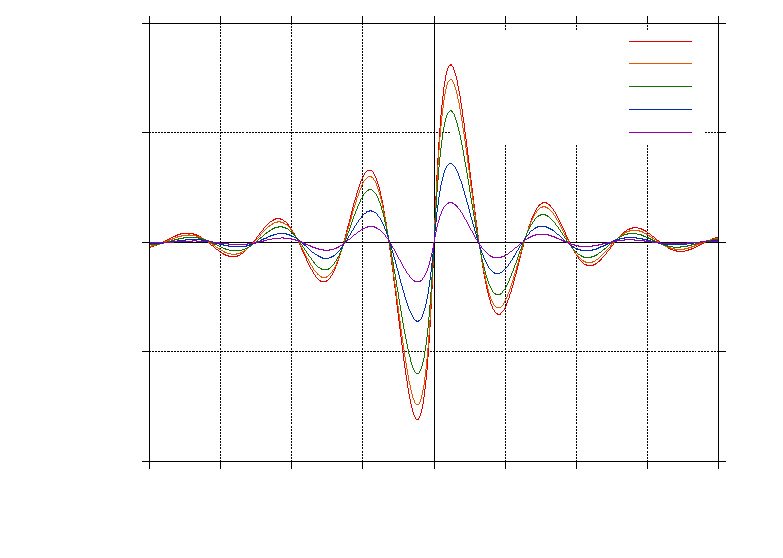
\includegraphics{Figures/CorrelationFunction/corfunc}}%
    \gplfronttext
  \end{picture}%
\endgroup
  
\caption{The real space correlation function $\braket{\psi_F(x)\psi_F(0)}$ is plotted as a function of $k_Fx$ for $T = 0$. Parameters: $(n_Ba_B^3)^{1/3} = 0.01$, $(n_Ba_{BF}^3)^{1/3} = 0.1$, $l_t = 0$, $\frac{m_B}{m_F} = 7/40$, $\frac{n_F}{n_B^{1/3}} = 0.215$, $v_F/c_0 = 0.33$. The red graph here corresponds to the red graph in figure \ref{fig.Deltakkdepend}.}  
\label{fig.pairwavefunction}  
\end{center}    
\end{figure}

\section{The mean field approximation revisited}
We are now in a position, where we can formulate the mean field approximation in a precise manner. In the mean field approximation of chapter \ref{Chapter4} we say, that $A_F(x,x') = \psi_F(x)\psi_F(x') - \braket{\psi_F(x)\psi_F(x')}$ has to be small with respect to the mean $\braket{\psi_F(x)\psi_F(x')}$. As we saw in the above subsection, $\psi_F(x)\psi_F(x')$ only depends on the difference $x-x'$. Hence we only investigate $A_F(x,0)$. 
To quantify the mean field approximation we calculate the variance of the stochastic operator $\psi_F(x)\psi_F(0)$:
\begin{equation}
\mathbb{V}[\psi_F(x)\psi_F(0)] = \braket{(\psi_F(x)\psi_F(0))^\dagger \psi_F(x)\psi_F(0)} - \left|\braket{\psi_F(x)\psi_F(0)}\right|^2. \nonumber  
\end{equation}

The calculation of this for $T = 0$ goes along the same lines as in the last subsection. We express $f_k, f_{-k}$ through the $\zeta$-operators and use $\zeta_k \ket{\text{S}}_0 = 0$. This leads to the following expression for $T = 0$:
\begin{equation}
\mathbb{V}[\psi_F(x)\psi_F(0)] = \frac{1}{\mathcal{L}^2}\sum_k \sin^2(kx)|v_{F,k}|^4. \nonumber
\end{equation}
Changing to integrals and dividing by the norm square of the mean value (the pair wave function), we get:
\begin{equation}
\frac{\mathbb{V} [\psi_F(x)\psi_F(0)] }{\left|\braket{\psi_F(x)\psi_F(0)}\right|^2} = \frac{2}{N_F}\frac{\int d\tilde{k} \sin^2(\tilde{k}\tilde{x})|v_{F,\tilde{k}}|^4}{\left| \int d\tilde{k} \sin( \tilde{k}\tilde{x} )\frac{ \Delta_{\tilde{k}} }{ 2E_{F,\tilde{k}} } \right|^2 },
\label{eq.RelativeVarianceSupefluidField}
\end{equation}
where $\tilde{k} = k/k_F$. In calculating this expression we have used, that $k_F \mathcal{L} = \pi n_F \mathcal{L} = \pi N_F$. This shows, that the variance relative to the mean value norm squared is proportional to $1/N_F$. Since we are considered a macroscopic number of particles $N_F \sim 10^{20}$, and so this ratio will be negligible. This specifies in detail what is meant by the mean field approximation made in chapter \ref{Chapter4}. We are thus assured, that the developed theory is selfconsistent. It is truly a satisfactory result to see explicitly, that the mean field approximation is intimately related to the number of particles in the system, and that it gets better and better as $N_F$ increases.  



